%% SOURCE: experiments/010-kuzmin-tmi/scripts/screen_diversity_audit.py -- per-gene counts from results/screen_diversity_per_gene.csv, panel verdict from results/screen_diversity_panel.csv, correlations from results/screen_diversity_summary.json; corrected panel from positive_panel_selection.py with the screen gate

\section{Correction: a record count is not support\secstatus{todo}}

The support gate in Section~3 counted trigenic training records and set the floor
at 200. \texttt{YER059W} passes it at 1{,}097. Every one of those records comes
from a single screen, and once that is corrected the positive signal in
\texttt{inference\_1} does not survive.

\subsection{What the gate missed\secstatus{todo}}

Kuzmin crosses a query double mutant against an array of single mutants, so a
gene's records are grouped by the query double they were measured under. Grouping
\texttt{YER059W}'s records that way gives one group. Its only query double is
\texttt{YER059W + YIL050W}, crossed against 1{,}097 array genes, and the gene
never appears as an array gene itself. The model has never seen it in any
combination not containing \texttt{YIL050W}.

The distribution over all 4{,}352 genes has a gap that makes the floor
insensitive: 2{,}339 genes were measured under 10 to 49 distinct screens and
1{,}171 under 200 or more, with only 11 in between. Eighty-eight genes, 2.0
percent, sit at exactly one screen, and their median record count is 1{,}046. A
record floor cannot see any of them.

\begin{table}[H]
\centering
\begin{tabular}{lrrl}
\toprule
Gene & records & distinct screens & \\
\midrule
\texttt{YER059W} & 1097 & 1   & fails \\
\texttt{YDR423C} & 1049 & 10  & fails \\
\texttt{YLR258W} & 1114 & 10  & fails \\
\texttt{YGL060W} & 1321 & 281 & passes \\
\texttt{YHR204W} & 288  & 288 & passes \\
\texttt{YKR028W} & 1323 & 295 & passes \\
\texttt{YPL181W} & 295  & 295 & passes \\
\texttt{YJR082C} & 796  & 296 & passes \\
\texttt{YHR003C} & 1356 & 297 & passes \\
\texttt{YGR121C} & 1413 & 315 & passes \\
\bottomrule
\end{tabular}
\caption{The proposed panel against a floor of 50 distinct screens. Record count
and screen count are nearly uncorrelated across these ten: \texttt{YHR204W} has
the fewest records and is measured under 288 screens, while \texttt{YER059W} has
the most and is measured under one.}
\end{table}

\subsection{The predictions track that one screen\secstatus{todo}}

Six of the seven \texttt{YER059W} partners in the panel were array genes in its
screen, with measured $\tau$ there of $+0.796$ for \texttt{YGR121C}, $+0.799$ for
\texttt{YPL181W}, $+0.585$ for \texttt{YGL060W}, $+0.523$ for \texttt{YBR028C},
$+0.472$ for \texttt{YHR003C} and $+0.430$ for \texttt{YPL089C}. A tier A triple
substitutes one of those partners for \texttt{YIL050W} and asks for a prediction.

Over the 2{,}730 \texttt{inference\_1} triples containing \texttt{YER059W} whose
two partners were both measured in that screen, the predicted $\tau$ correlates
with the partners' measured in-screen values at $0.495$ on their mean and
$0.599$ on their minimum.

That is consistent with the model reproducing one screen's values rather than
computing a three-way interaction, and it is not proof. The alternative is that
\texttt{YER059W} genuinely interacts positively with those partners, the screen
measured that correctly, and the prediction is right for the right reason. The
two are not separable without building the strains.

\subsection{The strong tier is this effect\secstatus{todo}}

Across \texttt{inference\_1}, 4.46 percent of triples contain a gene measured
under exactly one screen. Among the 39 triples predicted above $+0.08$ that rises
to 59.0 percent, and among the 15 above $+0.16$ to 86.7 percent, enrichments of
$13.2$ and $19.4$ times.

Applying the 50-screen floor to the selection and re-running it end to end, the
best available triple falls from $+0.662$ to $+0.069$, and 15 of 20 rather than
20 of 20 are positive under all three checkpoints. Ten times the signal was
carried by genes the screen structure cannot support.

\begin{figure}[H]
\centering
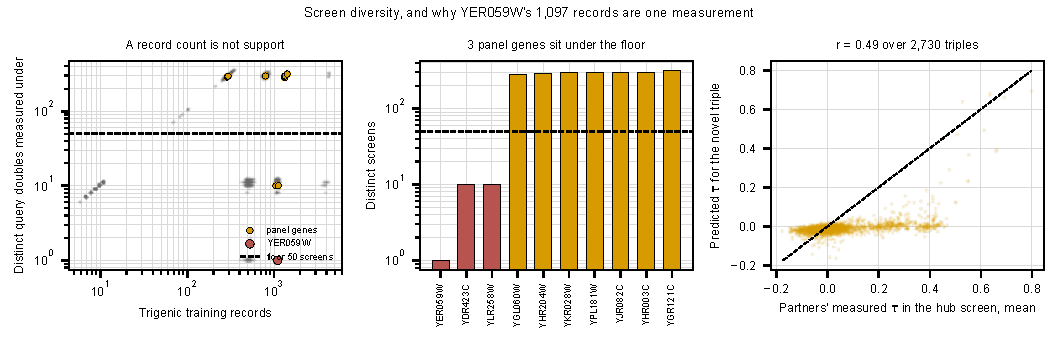
\includegraphics[width=\linewidth]{figures/screen_diversity_audit.pdf}
\caption{Record count against screen count, the panel's verdict, and predicted
$\tau$ for novel \texttt{YER059W} triples against the memorized values of their
partners. Generated by
\protect\file{experiments/010-kuzmin-tmi/scripts/screen_diversity_audit.py}.}
\end{figure}

\subsection{What this changes\secstatus{todo}}

The selection now carries \texttt{MIN\_DISTINCT\_SCREENS}, so the panel in
Section~4 is superseded by the gated one. The honest reading of the gated result
is that this model has no strong positive prediction on \texttt{inference\_1}
that does not rest on a gene measured under one or a few screens.

That does not make the round pointless, it changes what it tests. A panel whose
best prediction is $+0.069$ against a label standard deviation of $0.063$ is a
test of whether the model can rank at all near the noise floor, not a search for
a large effect. Deciding whether that is worth a plate is a judgment about cost,
and the alternative is to build the \texttt{YER059W} tier knowing it may measure
one screen's offset rather than an interaction.
